

\section{Overview}
\subsection{Compared systems}
GNN systems are designed to execute (and scale) GNN workloads. Some focus on single-node execution and optimizing data movement across memory hierarchy; some focus on distributed settings and optimizing network communications and graph partitioning. The usual goals are better runtime efficiency, measured as per-epoch training time, and data/model scalability, tested by the system capable of executing the workload without OOM issues. This is an emerging field, and many of these systems are still developing and changing rapidly.

Although there are many sub-branches in GNN study, the vast majority of these systems focus on the spatial-based methods, that is, recurrent GNNs and spatial-based graph convolutional neural networks (also known as GCNs). Majority of spatial methods can be expressed via a general update rule:
\begin{gather}
\label{eq:mp}
\mathbf{h}_v ^k = \psi ( \mathbf{x}_v^k, \gammasum_{u \in {\mathcal {N}}(v)} \phi(\mathbf{h}_v^{k-1}, \mathbf{h}_u^{k-1}, \mathbf{x}_{e_{vu}})),
\end{gather} 
where $\psi$, $\phi$, $\Gamma$ are potentially learnable and differentiable functions, $\Gamma$ is typically further required to be commutative and associative. $\psi$ is called the update function, $\phi$ the message function and $\Gamma$ the aggregate function. $\mathbf{h}_v^{k}$ is the node embedding for node $v$ at the $k$-th layer. $\mathcal {N}(v)$ is a function that returns all the neighbors for node $v$. $\mathbf{x}_{e_{vu}}$ is the edge feature.

\begin{figure*}[t]
 \centering
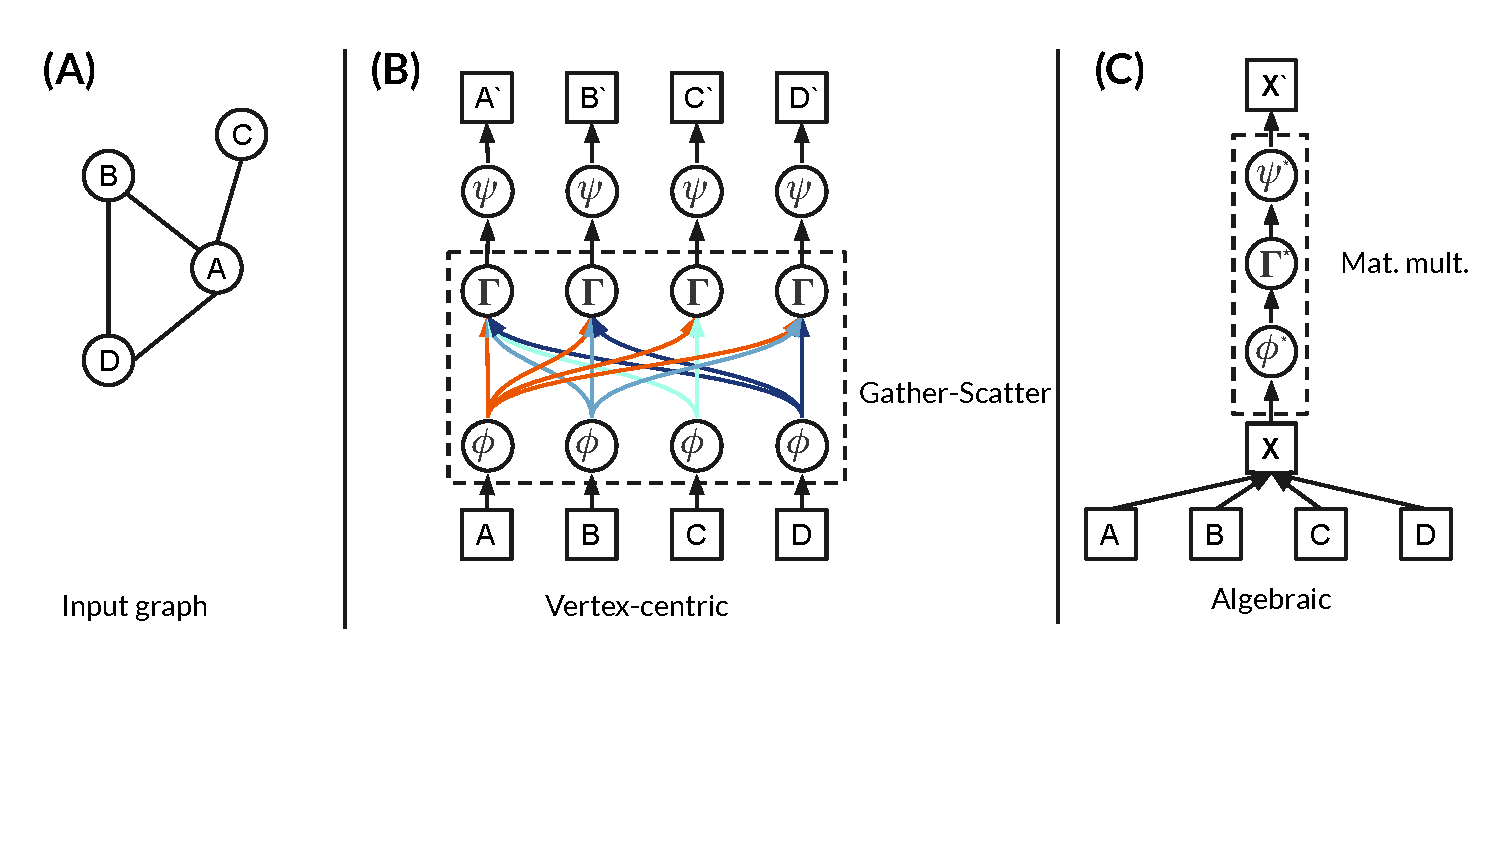
\includegraphics[width=0.70\textwidth]{./images/gnnsys.pdf}
 \caption{An example of two different approaches for GNN execution. (A): Input graph. (B): Vertex-centric approach. (C): Algebraic approach.}
 \label{fig:gnnsys}
\end{figure*}

\vspace{2mm}
\noindent \textbf{PyTorch Geometric (PyG)}  
Equation~\ref{eq:mp} fits in the paradigm of vertex-centric programming, which is a common programming model in the graph processing world~\cite{vertexcentric, powergraph, pregel} and is very easy to parallelize. One of the first GNN systems, PyG~\cite{pyg} follows this pattern and builds GNNs as dataflow graphs on top of PyTorch~\cite{torch}, a dataflow system. Figure~\ref{fig:gnnsys} (B) shows an example computational graph generated\footnote{Note this observation is based on the paper of PyG, in the recent versions of the release, PyG has implemented support for algebraic approach as well.}. Each (vectorized) operation is then put on a separate processor to achieve parallelism. Built on top of PyTorch, PyG can easily utilize the features PyTorch provides, such as autograd, GPU acceleration, etc. 

\vspace{2mm}
\noindent \textbf{Deep Graph Library (DGL) and DistDGL.}  
Arguably the most popular GNN system, DGL~\cite{dgl} takes a different approach for the GNN execution, especially for the message passing (gather-scatter) part. It takes an algebraic approach for the execution by expressing GNN as sparse matrix multiplications (SpMM). This is analogous to those algebraic approaches to general graph analytics tasks~\cite{graphla}.

Figure~\ref{fig:gnnsys} (C) gives an example of the algebraic approach taken by DGL; each step is summarized as linear algebra and executed as SpMM, which is executed via DGL's own specialized kernel. DGL is built upon existing deep learning systems, and the user can also write user-defined functions to extend the built-in functions. DGL describes itself as a framework-independent system, that is, independent of the underlying deep learning system. It has full support for several popular frameworks such as Tensorflow or PyTorch as backend. Backpropagation can also be done via another SpMM, and DGL functions are registered in the underlying deep learning framework to take advantage of autograd.

The algebraic approach opens possibilities of operator fusion. For many GNNs, the message function and aggregate function can be represented with purely matrix multiplications. Note in this form, the message function can be fused with the aggregation function, and there is no need to materialize the intermediate messages, thus saving space. For scalability, DGL goes for distributed processing as DistDGL~\cite{distdgl}.

\vspace{2mm}
\noindent \textbf{NeuGraph.}
NeuGraph~\cite{neugraph} is another GNN system built on top of a dataflow system and designed for a single-node multi-GPU setting. It extends the GAS~\cite{powergraph} programming model and partitions the graph into chunks. It feeds chunks instead of the full graph to GPU, avoiding GPU OOM issues for GNNs without sampling the data. After feedforward propagation, chunks are swapped back to the main RAM. There are also a series of processing order and scheduling challenges that it tries to solve. It further exploits GPU-to-GPU communication to avoid latencies of GPU-to-DRAM. 

\vspace{2mm}
\noindent \textbf{PaGraph.}
PaGraph~\cite{pagraph, pagraph2} also targets single-node multi-GPU settings and claims that the majority of the time (74\%) during GNN training is spent on data movement between the main RAM and GPU memory. Therefore, to reduce such data movement, they utilize the spare GPU memory to cache certain graph nodes' features statically. They select this set of cache based on the nodes' degree. They then proposed a GNN-aware graph partition scheme for multi-GPU support. This partition scheme would ensure that each partition contains all of the training graph nodes' K-hop neighbors by replication. In a subsequent work~\cite{pagraph2}, the authors also incorporated pipelining. PaGraph is built on top of DGL and PyTorch.

\vspace{2mm}
\noindent \textbf{AliGraph.} 
AliGraph~\cite{aligraph} is one of the early distributed GNN systems that come with only CPU support. The paper proposes a GNN training platform and a GNN algorithm to tackle real-world e-commerce graph analytics challenges. On the system side, they propose to store the graph structural information and node features data separately. AliGraph then uses indices to represent the node features, therefore reduces the storage cost. They then adopt an LRU cache to reduce access time for the most frequent graph nodes above a threshold based on their degrees. Furthermore, they adopt a lock-free distributed data structure (with cache) that facilitates graph sampling common in GNN training.

\vspace{2mm}
\noindent \textbf{ROC.} 
ROC~\cite{roc} is a distributed GNN system that attempts to boost both the efficiency and scalability of GNN training. Towards the former goal, it adopts an ML-based method for determining the graph partition. For the later pursuit of scalability, it proposes system DRAM spill when the GPU memory is insufficient to execute the GNN workload. ROC is built upon a custom-built DNN execution backend with customized CUDA kernels, FlexFlow~\cite{flexflow}.


\vspace{2mm}
\noindent \textbf{P$^{3}$.} P$^{3}$~\cite{pcube} is a distributed GNN system that proposes to use a ``hybrid" parallelism for GNN training. They argue that under the distributed setting, training time is dominated by communication time. They also claim that the bulk of communication happens during the first layer of GNNs. P$^{3}$ then proposes to 1. partition the graph structure and node features independently. 2. partition the node features uniformly along the dimensions. This way, they execute GNNs' first layer via model parallelism since each machine contains only several dimensions of the features. They then invoke all-to-all communications, let each machine pull all the needed features, and proceed as normal data parallelism for subsequent layers. This execution scheme would bring extra overhead compared to simple data parallelism, but the authors argue such overheads are compensated by the performance gain brought by communication reduction.



\vspace{2mm}
\noindent \textbf{DeepGalois.} 
DeepGalois~\cite{deepgalois} is a CPU-only distributed GNN system built on a graph processing system Galois~\cite{galois}. Additionally, it is also built on top of a series of existing graph partitioning and distributed communication frameworks. Because of these mature components, DeepGalois can support many graph partitioning schemes and can outperform distDGL. At the moment, there is not yet a full paper about DeepGalois, and no public release can be found.


\vspace{2mm}
\noindent \textbf{Neo4j, TigerGraph, and GraphScope.}
Both Neo4j~\cite{neo4j} and TigerGraph~\cite{tigergraph} are graph DBMSes that have some GNN training capabilities. GraphScope~\cite{graphscope} is a recent graph processing system that primarily focuses on traditional graph analytics such as community detection, paths and connectivity, and centrality, but it also has extensible connectors to other systems to enable GNN processing.

Neo4j has implemented a specialized in-memory graph store for GNNs and other more advanced analytics. It first moves data from the graph DB to this store at runtime and invokes a custom-built library for building GNN models and SGD training. As of now, it only supports GraphSage. 

GraphScope takes a similar approach to Neo4j by moving data to a dedicated GNN facility. But instead of a custom-built framework, it can utilize TensorFlow and provides a few pre-built implementations of several popular GNNs.

TigerGraph, similar to Neo4j, only provides limited GNN support for simple GCNs. However, it takes a different approach by also storing all the NN neurons in graph DB. As mentioned above, such GNNs can be captured under the GAS abstraction. This way, the GNN can be expressed mostly in the form of graph DB operators instead of the external library's dataflow operators. Forward and backward propagation can be written using TigerGraph's DSL: GSQL. Gradient computing is implemented in the form of UDFs.


\subsection{Other related systems}

\vspace{2mm}
\noindent \textbf{Custom-built, Specialized GNN Frameworks.} Due to the lack of support for GNNs from the commonly used deep learning frameworks such as TensorFlow and PyTorch and various other reasons, many ML researchers sought to build their own library for their specific GNNs/applications~\cite{agl, graphsage}. These frameworks usually are very specific and have little consideration for system performances such as efficiency and scalability. Therefore, they are excluded from our discussion.


\vspace{2mm}
\noindent \textbf{Knowledge Graph Embedding Systems.} There exists a connected, yet still different field of knowledge base graph embedding systems~\cite{marius, dgl-ke, pbg, lightne}. The goal of such systems is to obtain embeddings for each node within the graph. However, instead of training a GNN and using its internal latent node representations as node embeddings, these methods train the embeddings directly using the graph's structural information. They do not use GNNs, and they usually work on graphs that are not featured, i.e., node and edge features unavailable. These systems also face efficiency and scalability challenges, mostly brought by the sheer size of knowledge base graphs instead of GNNs. Many of them sought to use distributed processing, intelligent caching, and disk-aware processing to tackle these problems. Some of the techniques can be adopted for GNN systems, but many are specific to knowledge graph embedding workloads.

%----------------------------------------------
\begin{table*}[h]
\caption{Overview of comparisons.}
\scalebox{0.58}{
\huge{
\begin{tabular}{@{}ccccccccccc@{}}
\toprule
\multirow{2}{*}{} & \multirow{2}{*}{License} & \multirow{2}{*}{GPU} & \multicolumn{4}{c}{Efficiency}                     & \multicolumn{2}{c}{Scalability} & \multirow{2}{*}{Expressibility} & \multicolumn{1}{l}{\multirow{2}{*}{Memory Hierarchy}} \\ \cmidrule(lr){4-9}
         &             &           & Data movement & Communication & Training & \multicolumn{1}{c|}{Overall} & Distributed   & Sampling   &                 & \multicolumn{1}{l}{}                 \\ \midrule
PyG~\cite{pyg}        & Open           & Yes         & -       & N/A      & +    & -    & No        & Generic   & GAS               & GPU-only                       \\
DGL~\cite{dgl, distdgl}        & Open           & Yes         & -       & -       & +    & -    & Yes       & Generic   & MM               & GPU-only                       \\
NeuGraph~\cite{neugraph}     & N/A           & Yes         & ++      & N/A      & +    & +    & No        & GD      & GAS               & Main-aware                      \\
PaGraph~\cite{pagraph, pagraph2}      & Open           & Yes         & ++      & N/A      & +    & ++   & No        & SGD     & MM               & Main-aware                      \\
AliGraph~\cite{aligraph}     & Open           & No          & +       & +       & -    & -    & Yes       & SGD     & GAS               & Main-only                       \\
ROC~\cite{roc}        & Open           & Yes         & +       & +       & +    & ++   & Yes       & GD      & GAS               & Main-aware                      \\
P$^{3}$~\cite{pcube}      & N/A           & Yes         & -       & ++      & -{}-    & ++   & Yes       & SGD     & MM*               & GPU-only                       \\
DeepGalois~\cite{deepgalois}    & N/A           & No          & -       & +       & -    & +    & Yes       & GD      & GAS               & Main-only                       \\
Neo4j~\cite{neo4j}       & Mixed          & No          & -{}-      & N/A      & -    & -{}-   & No        & SGD     & ?                & Main-only?                      \\
TigerGraph~\cite{tigergraph}    & Closed          & No          & -       & -       & -    & -    & Yes?       & GD?     & GAS?              & Main-only?                      \\
GraphScope~\cite{graphscope}    & Open           & Yes         & -{}-      & ?       & -    & -    & No?       & Generic?   & ?                & GPU-only?                       \\ \bottomrule
\end{tabular}
}
}
\label{tab:comp}
\end{table*}

\vspace{-2mm}
\section{Comparisons of GNN systems}
An overview of all the systems compared is shown in Table~\ref{tab:comp}.
\label{sec:comp}
\subsection{Availability (licenses)}
To benchmark and development on top of these systems, ideally, we want them to be free and open-sourced.


\vspace{2mm}
\noindent \textbf{Open-source license.}
The majority of the GNN systems surveyed are open-sourced; exceptions are below.


\vspace{2mm}
\noindent \textbf{Proprietary license.}
TigerGraph is released under a proprietary license; the free version comes with a limitation of graph storage size. Neo4j, on the other hand, has both a free open-sourced version that comes with various limitations and a paid commercial version.

\vspace{2mm}
\noindent \textbf{Not available.}
There are no public releases found for NeuGraph, DeepGalois, and P$^3$.




\subsection{Accelerator (GPU) Support}
With GPU support, two extra problems arise 1. efficient data movement between main memory and GPU memory 2. memory management to prevent crashes, as GPU RAM is usually more limited. Not all systems have GPU support.

\vspace{2mm}
\noindent \textbf{GPU-supported.} PyG, DGL, NeuGraph, PaGraph, ROC, P$^{3}$, and GraphScope all support GPU training. Among these, PyG, DGL, and ROC have custom-built GPU kernels for GNNs. The rest are based on existing systems for GPU support.

\vspace{2mm}
\noindent \textbf{CPU-only.} AliGraph, DeepGalois, Neo4j, and TigerGraph are CPU-only at the moment.

\subsection{Runtime Efficiency (Speculated)}
This section is based on the published results from the papers. These results are not directly comparable, as they are not done on the same platform, nor the same datasets/models. Hence, currently, without more rigorous tests, the efficiency can only be speculated. There are many aspects to the runtime efficiency: 1. data movement efficiency across memory hierarchy, pipelining, and efficiency latency hiding. 2. The network communication efficiency, graph partitioning quality, cache, and novel parallelization schemes for distributed systems. 3. actual training efficiency, i.e., runtime spent in GPU. 

In the literature, the more common baselines are DGL and PyG. Between the two, both of their papers claim to be faster and more scalable; it is unknown if they have a substantial performance gap.

\vspace{2mm}
\noindent \textbf{Data movement efficiency.}
A few systems have efforts to optimize the data movement, especially the DRAM-GPU movement. The common techniques are caching and pipelining. NeuGraph, ROC, and PaGraph all adopt some form of caching to reduce the data movement and try to overlap computation with data transfer. NeuGraph further exploits opportunities for GPU-GPU data movement.

\vspace{2mm}
\noindent \textbf{Network communication efficiency.} Networking becomes part of the problem when distributed processing comes to the picture. AliGraph and ROC both consider graph partitioning algorithms and caching to boost data locality and reduce communication. DeepGalois relies on the underlying graph processing software stack for optimized graph partitioning and distributed communication. P$^{3}$, on the other hand, proposes a parallel execution scheme that mixes model parallelism and data parallelism to reduce communications.

\vspace{2mm}
\noindent \textbf{Training efficiency.} Most of the systems should have close performance in this department. However, as PyG, DGL, NeuGraph, and ROC all have their custom-made GPU kernels for graph propagation, it is unknown which one is the winner as no such drill-down benchmark is currently available. In addition, P$^3$ adopts a model parallelism training scheme that is different from all other systems, and this scheme, although it may save communications, but would likely add overheads to training.



\subsection{Scalability (Speculated)}
Due to the neighborhood explosion problem and the scale of large graphs, GNNs suffer from scalability issues as the entire graph is usually much larger than the GPU memory can hold. A series of algorithmic efforts, focusing on sampling, have been proposed to mitigate this issue. However, even with mini-batch SGD and sampling over the data, it is claimed that many of such workloads can still face scalability issues. Common techniques include 1. distributed processing that enables multi-GPUs, and 2. spilling to the main RAM to prevent OOM. Distributed processing would lead to topics such as graph partitioning, network communication, and parallel schemes. Spilling to the main RAM is tightly connected to topics such as caching and pipelining.

\vspace{2mm}
\noindent \textbf{Distributed processing.} DGL, ROC, DeepGalois, P$^{3}$, AliGraph, and TigerGraph can all support distributed GNN training. PyG, NeuGraph, PaGraph are single-node systems.

Neo4j and GraphScope are unknown if their export-based methods can be made distributed. Apart from this, Neo4j is currently still primarily a single-node and not fully distributed graph DB\footnote{https://neo4j.com/news/neo4j-going-distributed-with-graph-database/}.

\vspace{2mm}
\noindent \textbf{Graph sampling.} 
There are mainly two categories of systems in terms of graph sampling and training scheme: full-batch and mini-batch.
\begin{enumerate}
\item \textbf{Full-batch. (Gradient descent and unsampled)}.
The first try to optimize for full-batch training of GNNs, i.e., naively, would require the entire graph to fit in the main or GPU RAM. This category includes NeuGraph, ROC, and DeepGalois. TigerGraph currently has some support for GCNs and can work under a full-batch setting. However, it is unknown to what extend it is scalable.
\item \textbf{Mini-batch. (SGD and sampled)}. The second category assumes a mini-batched and sampled graph. Therefore they only require a mini-batch of data to fit in the RAM. This category includes PaGraph, AliGraph, and P$^{3}$. Neo4j only supports GraphSage algorithm at the moment, which is a mini-batch method with sampling. 
\item \textbf{Generic. (Unspecified)}. These systems claim to be generic or not specifically optimized for any one particular setting. It includes DGL, PyG, and GraphScope.
\end{enumerate}
Technically the first category should also work under the mini-batched setting, but the reverse may not be true.  


\subsection{GNN Expressibility}
\begin{figure}[t]
 \centering
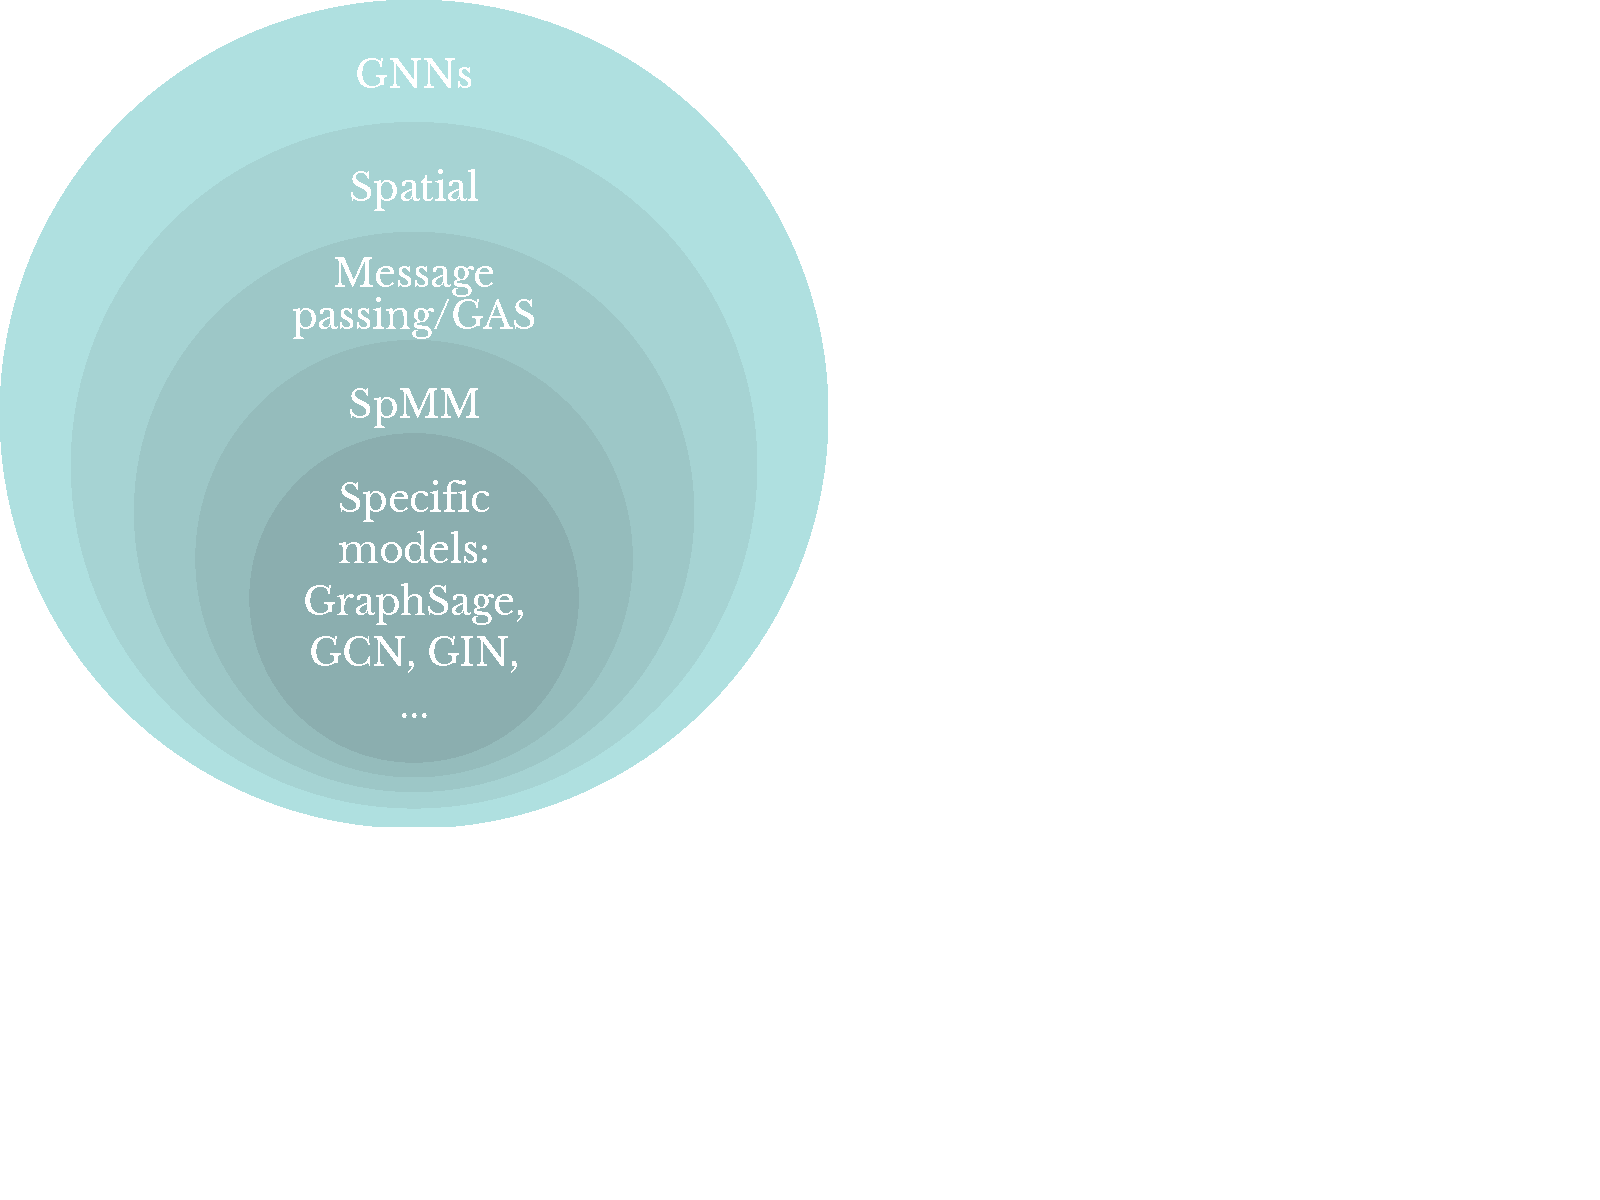
\includegraphics[width=0.35\textwidth]{./images/venn_diagram.pdf}
 \caption{Venn diagram of different scopes of GNNs.}
 \label{fig:venn}
\end{figure}


We now evaluate how generic these systems are and the family of GNN models that can be expressed/executed by these systems. Figure~\ref{fig:venn} shows the overall scope of comparisons. 
\begin{itemize}
\item First, all of these systems are primarily designed for spatial methods; most of the spectral-based GNNs are well-supported, except a few methods like ChebNet~\cite{chebnet} that bridge the spectral- and spatial-based GNNs. 
\item Furthermore, many systems are based on the message passing interface shown in Equation~\ref{eq:mp}, also can be captured under the GAS framework. Such systems include PyG, NeuGraph, AliGraph, ROC, and DeepGalois.
\item DGL further requires the GNN to be expressible as matrix multiplications. PaGraph is built on top of DGL, so it shares the same expressibility. On the other hand, for P$^{3}$ to show performance gain, the update function of the model needs to be model-parallelizable, which usually means linear operations/simply matrix multiplications.
\item Neo4j, TigerGraph, and GraphScope did not focus on the GNN expressibility and are unknown how general their programming interface is, or they do not have a generic programming interface for expressing various GNN models. 
\end{itemize}

\subsection{Span of Memory Hierarchy}
We now inspect each system's usage of the different memory hierarchy, from accelerator memory to disk. Generally speaking, the wider the span is, the better the system can scale with large models and data. Not all systems support GPUs, so some of them do not have GPU RAM. But as more tiers hierarchy are involved, the latencies grow and the demand for buffering and memory management also grow.

\vspace{2mm}
\noindent \textbf{GPU RAM Only.} DGL, PyG, and P$^{3}$ are GPU RAM only, meaning they require the full graph/minibatch to fit in the memory.


\vspace{2mm}
\noindent \textbf{Main RAM Only/Aware.} AliGraph and Neo4j are main RAM only. NeuGraph, PaGraph, and ROC all utilize the main memory and spill intermediate results to it. They have different strategies to handle the main-memory to GPU data movement. All of the above require the data, GNN model, and intermediate results to fit in the main memory.

\vspace{2mm}
\noindent \textbf{Disk Aware.} At the moment, there are no systems that explicitly claim that they are disk aware. Neo4j and TigerGraph, as graph DBs, have disk spilling capability for the DB part. However, neo4j processes GNN workloads in a strictly in-memory store, while it is unclear whether TigerGraph can spill GNN intermediate states to disk. GraphScope, on the other hand, relies on external libraries for GNN execution and can be flexible.





